A tester consists of a validator and a test harness.  Chapters~\ref{chap:theory}
and \ref{chap:practices} have explained the validator's theory and practices.
This chapter presents a language-based design for test harnesses.  I'll show how
to generate and shrink test inputs effectively, addressing inter-execution
nondeterminism.

\autoref{sec:harness-overview} provides a brief overview of how test harnesses
work.  \autoref{sec:heuristics} explains how to write heuristics to generate
interesting test inputs.  \autoref{sec:shrinking} then shows how to keep the
test inputs interesting among different executions in the shrinking process.

\section{Overview}
\label{sec:harness-overview}
\begin{figure}
  \centering
  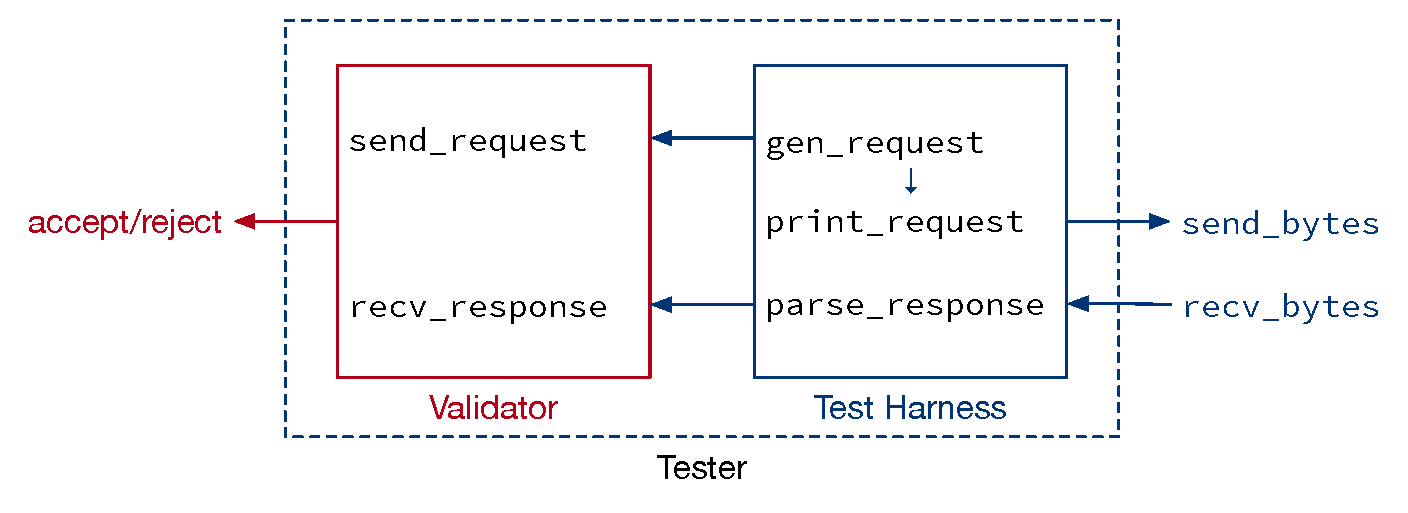
\includegraphics[width=.9\textwidth]{figures/harness-outline}
  \caption{Tester architecture outline.}
  \label{fig:overview}
\end{figure}

This section introduces the abstract architecture of an interactive tester,
using the networked server as an example.  I'll present a na\"ive implementation
of the test harness, which will be improved in the following sections.

The test harness interacts with the environment and provides the observations
for the validator.  The validator may represent requests and responses as
abstract datatypes for the convenience of specification.  The test harness
translates these abstract representations into bytes transmitted on the
underlying channel.

As shown in \autoref{fig:overview}, when the validator wants to observe a sent
request, the harness generates the request and encodes it into bytes to send.
Conversely, when the validator wants to observe a received response, the harness
receives bytes from the environment and decodes them into abstract messages.

\begin{figure}
\begin{lstlisting}[numbers=left]
Definition gen_packet: IO concrete_packet :=
  src          <- random_conn;;
  method       <- oneof [Get; Put];;
  target       <- random_path;;%\label{line:random-path}%
  precondition <- oneof [IfMatch, IfNoneMatch];;
  etag         <- random_etag;;
  payload      <- random_string;;
  ret { Source      := src;
        Destination := server_conn;
        Data        := inr { Method     := method;
                             TargetPath := target;
                             Headers    := [(precondition, etag)];
                             Payload    := payload
                           }
      }.
\end{lstlisting}
\caption{Na\"ive generator for HTTP requests.}
\label{fig:naive-generator}
\end{figure}

A generator is a randomized program that produces test inputs.  One example is
the \ilc{gen_packet} function in \autoref{fig:execute}.  The HTTP packet
generator can be na\"ively implementation as shown in
\autoref{fig:naive-generator}.  It fills in the request's fields with arbitrary
values, and has limited coverage of the SUT's behavior.  This is because the
request target and ETags are both generated randomly, but a request is
interesting only if its ETag matches its target's corresponding resource stored
on the server.  A randomly generated request would result in 404 Not Found and
412 Precondition Failed in almost all cases.

To reveal more interesting behavior from the SUT, we should tune the generator's
distribution to emphasize certain patterns of the test input.  For example, if
the tester knows the set of paths where the server has stored resources, then it
can generate more paths that correspond to existing resources; if the tester has
observed some ETags generated by the server, then it can include these ETags in
future requests.  In the next section, I'll explain how to implement such
heuristics in ITree-based testers.


\section{Heuristics for Test Generation}
\label{sec:heuristics}
This section implements heuristics for generating test inputs.  I'll use the
HTTP tester as an example to show how to make requests more interesting by
parameterizing them over the model state (\autoref{sec:heuristic-state}) and the
trace (\autoref{sec:heuristic-trace}).

\subsection{State-based heuristics}
\label{sec:heuristic-state}
\paragraph{Motivation}
The model state may instruct the test generator to produce more interesting test
inputs.  For example, consider the \ilc{random_path} generator in
\autoref{line:random-path} of \autoref{fig:naive-generator}.  One way to improve
it is to generate more paths that have corresponding resources on the server:
\begin{coq}
  Definition gen_path (state: list (path * resource)) : IO path :=
    let paths: list path := map fst state in
    freq [(90, oneof paths);
          (10, random_path)].
\end{coq}

Here I modify the server model's state type \ilc{sigma} from \ilc{(path ->
  resource)} in \autoref{fig:if-match-server} into \ilc{(list (path *
  resource))}, which allows the generator to access the list of all \ilc{paths}
  in the server state.  The generator chooses from these existing paths in 90\%
  of the cases, as assigned by the \ilc{freq} combinator.  The remaining 10\%
  are still generated randomly, to discover how the SUT handles nonexistent
  paths.

For the \ilc{gen_packet} generator in \autoref{fig:naive-generator}, replacing
its \ilc{random_path} with the improved \ilc{gen_path} would generate more
interesting request targets.  This requires the \ilc{gen_packet} function to
carry the server state to instantiate \ilc{gen_path}.

As shown in \autoref{fig:backtrack}, the \ilc{GenPacket} generator is triggered
when the tester wants to observe a packet from itself to the SUT.
\autoref{fig:symbolic-observer} then shows that such \ilc{FromObserver} expectation
happens when the symbolic model \ilc{Send}s a packet.  Such a \ilc{Send} event
only happens when the server wants to receive a packet in
\autoref{fig:net-compose}.  The \ilc{Recv} events are triggered by the server
model in \autoref{fig:if-match-server}, which iterates over the server state
\ilc{sigma}.

\paragraph{Implementation}
To expose the server state to the request generator, I extend the symbolic
server model's \ilc{Recv} event type on Page~\pageref{def:symbolic-qae} to
include the server state:
\begin{coq}
  Variant qaE: Type -> Type :=
    Recv : sigma      -> qaE packet
  | Send : packet -> qaE unit.
\end{coq}

Now when the server wants to receive a request, it triggers \ilc{(Recv state)},
where \ilc{(state: sigma)} contains the server's paths and resources at that
point.  The \ilc{state} argument is then carried to the generator, by adding
parameters to the event types along the interpretation:
\begin{coq}
  Variant netE: Type -> Type :=
    Emit  : packet -> netE unit
  | Absorb: sigma      -> netE packet.

  Variant observeE : Type -> Type :=
    FromObserver   : sigma -> observeE concrete_packet
  | ToObserver     : observeE concrete_packet.

  Variant genE: Type -> Type :=
    GenPacket : sigma -> genE concrete_packet
  | GenBool   : genE bool.

  Definition gen_packet: sigma -> IO concrete_packet.
\end{coq}

\begin{figure}
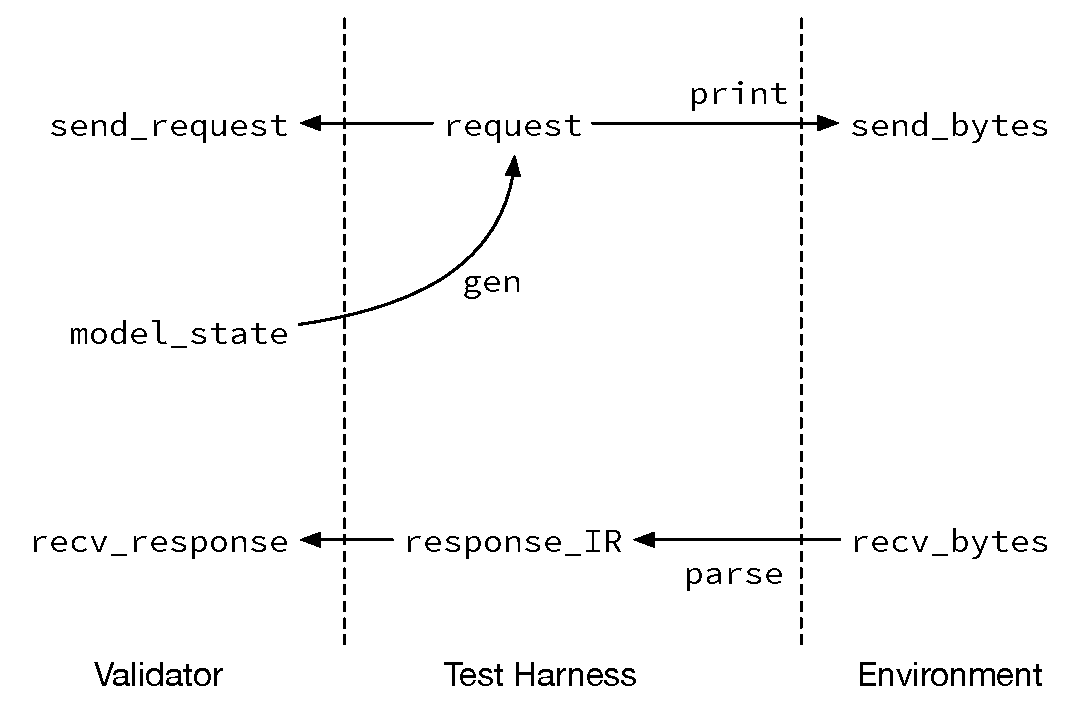
\includegraphics[width=.6\linewidth]{figures/stategen}
\caption{State-based heuristics.}
\label{fig:stategen}
\end{figure}

As a result, when instantiating the \ilc{(GenPacket state)} event in
\autoref{fig:execute}, we can feed the \ilc{gen_packet} function with argument
\ilc{state}, so that \ilc{gen_path} can generate interesting paths based on the
server state.  \autoref{fig:stategen} illustrates this state-based heuristics.
It refines the test harness box in \autoref{fig:overview}, and will be extended
with trace-based heuristics in the next subsection.

\subsection{Trace-based heuristics}
\label{sec:heuristic-trace}

When the SUT makes internal choices, \eg, generating ETags, the
specification represents them as symbolic variables.  These variables' concrete
values are not stored in the specification state, but may be observed during
execution.  For example, when an HTTP server responds to a GET request, it might
include the resource's ETag as shown in \autoref{sec:internal-nondeterminism}.

To improve the generator in \autoref{fig:naive-generator}, we can generate
interesting ETags based on the trace produced during execution.  The trace is a
list of packets sent and received by the tester, and the packets' payloads may
include responses that have an ETag field.  The \ilc{gen_etag} function
emphasizes ETags that were observed in the trace, which are more likely to match
those generated by the SUT:
\begin{coq}
  Definition gen_etag (trace: list concrete_packet) : IO string :=
    let etags: list string := tags_of trace in
    freq [(90, oneof etags);
          (10, random_etag)].
\end{coq}

To utilize this improved generator for ETags, the tester needs to record the
trace of packets sent and received.  This is done by modifying the \ilc{execute}
function in \autoref{fig:execute}, adding an accumulator called ``\ilc{trace}''
as the recursion parameter:
\begin{coq}
  Fixpoint execute (fuel: nat) (trace: list concrete_packet)
                   (m: itree tE void) : IO bool :=
    match fuel with
    | S fuel' =>
      match m with
      | Impure e k =>
        match e with
        | (ClientSend q|) => client_send q;;
                             execute fuel' (trace ++ [q]) (k tt)
        | (ClientRecv|)   => oa <- client_recv;;                             
                             let trace' := match oa with
                                           | Some a => trace ++ [a]
                                           | None   => trace
                                           end in
                             execute fuel' trace' (k oa)
        | (|GenPacket state|) => pkt <- gen_packet state trace;;
                                 execute fuel' trace (k pkt)
        ... (* similar to %\autoref{fig:execute}% *)
\end{coq}
%% \lys{\ilc{trace ++ [q]} is indeed less inefficient than storing a reversed trace,
%% but this code is to show the concept of ``appending'' requests and responses to
%% a trace, and assumes that readers have the ability of optimizing its
%% performance.}

When the tester sends or receives a packet, the packet is appended to the
runtime \ilc{trace}.  Then the \ilc{gen_packet} generator can take the trace
accumulated so far and feed it to the ETag generator:
\begin{coq}
  Definition gen_packet (state: sigma) (trace: list concrete_packet) :=
    target <- gen_path state;;
    etag   <- gen_etag trace;;
    ... (* same as %\autoref{fig:naive-generator}% *)
\end{coq}

\begin{figure}
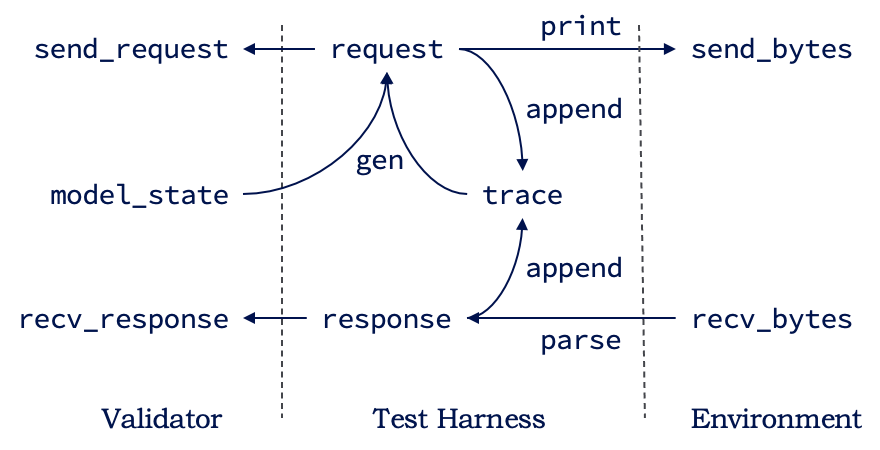
\includegraphics[width=.7\linewidth]{figures/gen}
\caption{Combining state-based and trace-based heuristics.}
\label{fig:gen}
\end{figure}

Now we can generate interesting test inputs by combining state-based and
trace-based heuristics, as shown in \autoref{fig:gen}.  In the next section,
I'll further extend this framework and shrink the test inputs while keeping them
interesting, addressing inter-execution nondeterminism.


\lys{Under construction:}

\section{Shrinking Interactive Test Inputs}
\label{sec:shrinking}

\autoref{fig:shrink} shows the test harness architecture for networked
servers.  This framework involves four languages: (1) An {\em
  application representation} (AR) which provides flexible abstraction
for encoding the validation logic per protocol under test; (2) {\em
  Bytes} that the tester interacts with the SUT over network; between
them, (3) The {\em intermediate representation} (IR) for encoding the
trace in an application-independent way; and (4) The {\em symbolic
  representation} called ``J-expressions'' (Jexp) which encodes the
input generated and shrunk by the test harness.

\begin{figure}
  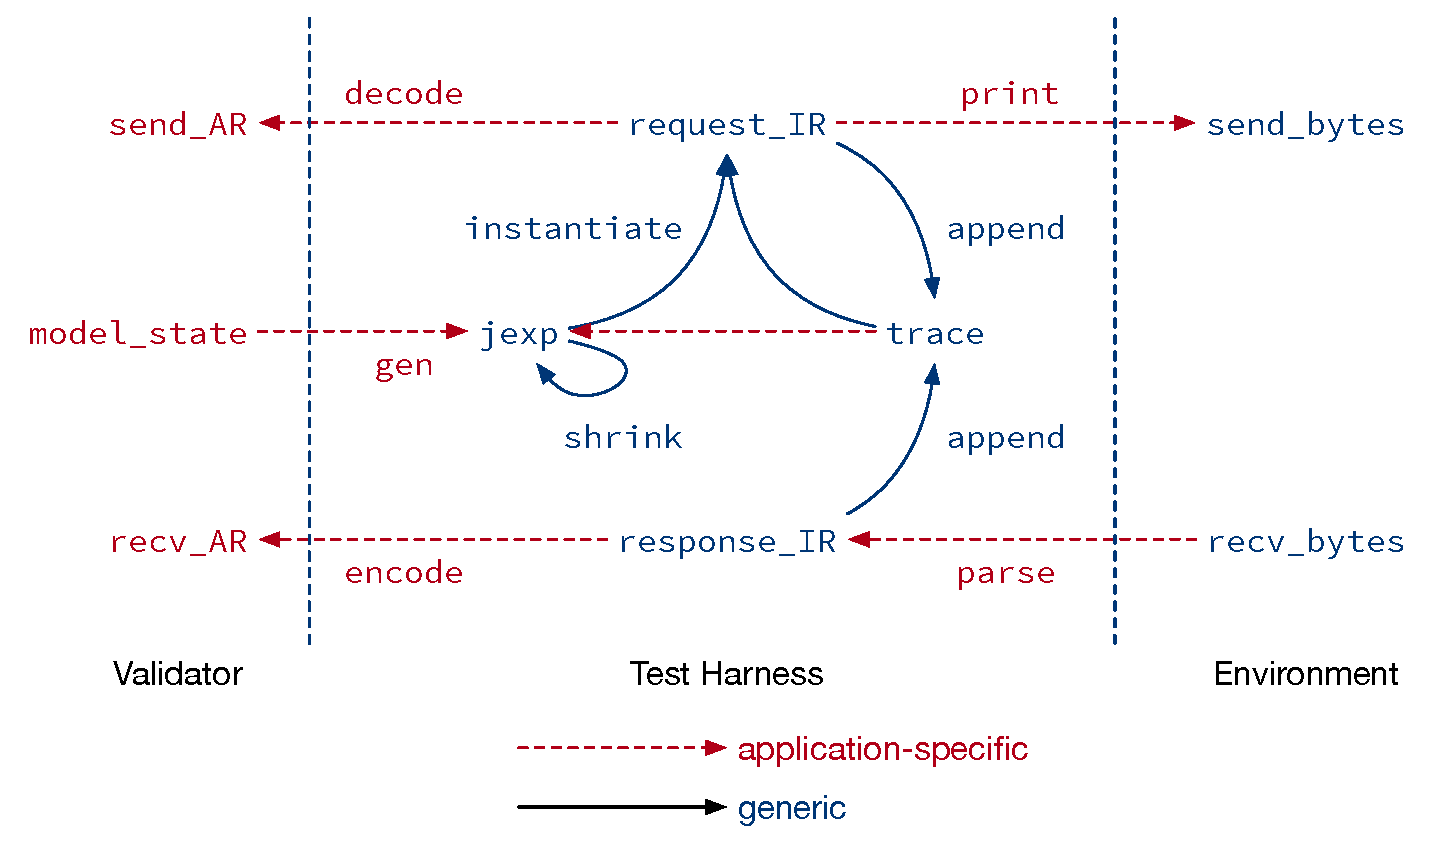
\includegraphics[width=.8\textwidth]{figures/shrink}
  \caption{Test harness architecture.  The test harness first generates
    J-expressions based on the model state provided by the validator.  The
    J-expression is a symbolic expressions that are instantiated by the trace
    into requests' IR.  When a violation is detected, the failing Jexp is shrunk
    into sub-expressions, and instantiated by the trace in new runs.  The dotted
    arrows are application-specific algorithms, while the solid arrows are
    generic over all protocols.}
  \label{fig:shrink}
\end{figure}

\section{Intermediate representation language}
The purpose of introducing an IR in this framework is to enable a generic method
for generating requests that refer to specific fields in the trace.  For
example, when testing conditional HTTP requests, the generator wants to include
``a precondition that uses the ETag field of a previous response''; when testing
an online store, the generator wants to provide ``an order ID that the server
has mentioned before''.

The IR in this framework is JSON, which allows syntax trees to be arbitrarily
wide and deep, and provides sufficient flexibility for network protocols in
general.  The J-expression is an extension of JSON that can refer to specific
fields in the trace:
\[\begin{array}{r@{\;}l}
\mathsf{JSON^T}\triangleq&\mathsf T\mid\{\mathsf{object^T}\}\mid[\mathsf{array^T}]\mid\mathsf{string}\mid\Nat\mid\Bool\mid\mathsf{null}\\
\mathsf{object^T}\triangleq&\nil\mid\mathsf{"string": JSON^T,object^T}\\
\mathsf{array^T}\triangleq&\nil\mid\mathsf{JSON^T,array^T}\\
\mathsf{IR}\triangleq&\mathsf{JSON^{IR}}\\
\mathsf{Jexp}\triangleq&\mathsf{JSON^{\Jref{\mathit{label}}{\mathsf{Jpath}}{\mathit{function}}}}\\
&\text{where }\mathit{label}\in\Nat,\mathit{function}\in\mathsf{IR}\to\mathsf{IR}\\
\Jpath\triangleq&\This\mid\Jpath\Number\mathit{index}\mid\Jpath\At\mathit{field}\\
&\text{where }\mathit{index}\in\Nat,\mathit{field}\in\mathsf{string}
\end{array}\]

The extended syntax
``$\Jref{\mathit{label}}{\mathsf{Jpath}}{\mathit{function}}$'' is a symbolic
expression that, given a runtime trace, can compute an IR of the request.  For
example, J-expression
``$\Jref{3}{\This\At\mathtt{"orders"}\Number2}{\mathtt{id}}$'' can be
pronounced: ``Look at the message labelled 3 in the trace, its `order' field
should be an array.  Find the 2nd element in that array, and use it
\ilc{id}entically (as-is).''  Such representation enables the test harness to
shrink counterexamples (encoded in Jexp) in a protocol-independent way.


\begin{figure}
  \begin{lstlisting}[style=customcoq]
    Example response1 : http_response :=
      Response (Status (Version 1 1) 200 (Some "OK"))
               [Field "ETag" "tag-foo";
                Field "Content-Length" "11"]
               (Some "content-bar").

    Example response2 : store_response :=
      Response__ListOrders [(233, (12, 100, 34, 500));
                            (996, (56, 400, 78, 20))].
  \end{lstlisting}
  \begin{minipage}[t]{.4\textwidth}
    \begin{lstlisting}[style=json]
      {
        "version": {
          "major": 1,
          "minor": 1
        },
        "code": 200,
        "reason": "OK",
        "fields": {
          "ETag": "tag-foo",
          "Content-Length": "11"
        },
        "body": "content-bar"
      }
    \end{lstlisting}
  \end{minipage}%
  \begin{minipage}[t]{.4\textwidth}
    \begin{lstlisting}[style=json]
      {
        "code": 200,
        "orders": [
          {
            "ID": 233,
            "BuyerID": 12,
            "BuyAmount": 100,
            "SellerID": 34,
            "SellAmount": 500
          },
          {
            "ID": 996,
            "BuyerID": 56,
            "BuyAmount": 400,
            "SellerID": 78,
            "SellAmount": 20
          }
        ]
      }
    \end{lstlisting}
  \end{minipage}
  \caption{Application message example for HTTP and online store protocols, and
    their corresponding intermediate representation}
  \label{fig:ir}
\end{figure}

To represent the correspondence between requests and responses, the trace labels
each message, and the request-response pair have the same label.
\autoref{fig:trace} shows a trace of messages sent and received by the tester
client.

\begin{figure}
  \begin{minipage}{.5\textwidth}
    \begin{lstlisting}[style=json]
      [
        {
          "label": 10,
          "message": {
            "method": "GET",
            "path": "index.html"
          }
        },
        {
          "label": 20,
          "message": {
            "method": "DELETE",
            "path": "index.html"
          }
        },
        {
          "label": 20,
          "message": {
            "code": 204,
            "reason": "No Content",
          }
        },
        {
          "label": 10,
          "message": {
            "code": 410,
            "reason": "Gone"
          }
        }
      ]
    \end{lstlisting}
  \end{minipage}%
  \begin{minipage}{.5\textwidth}
    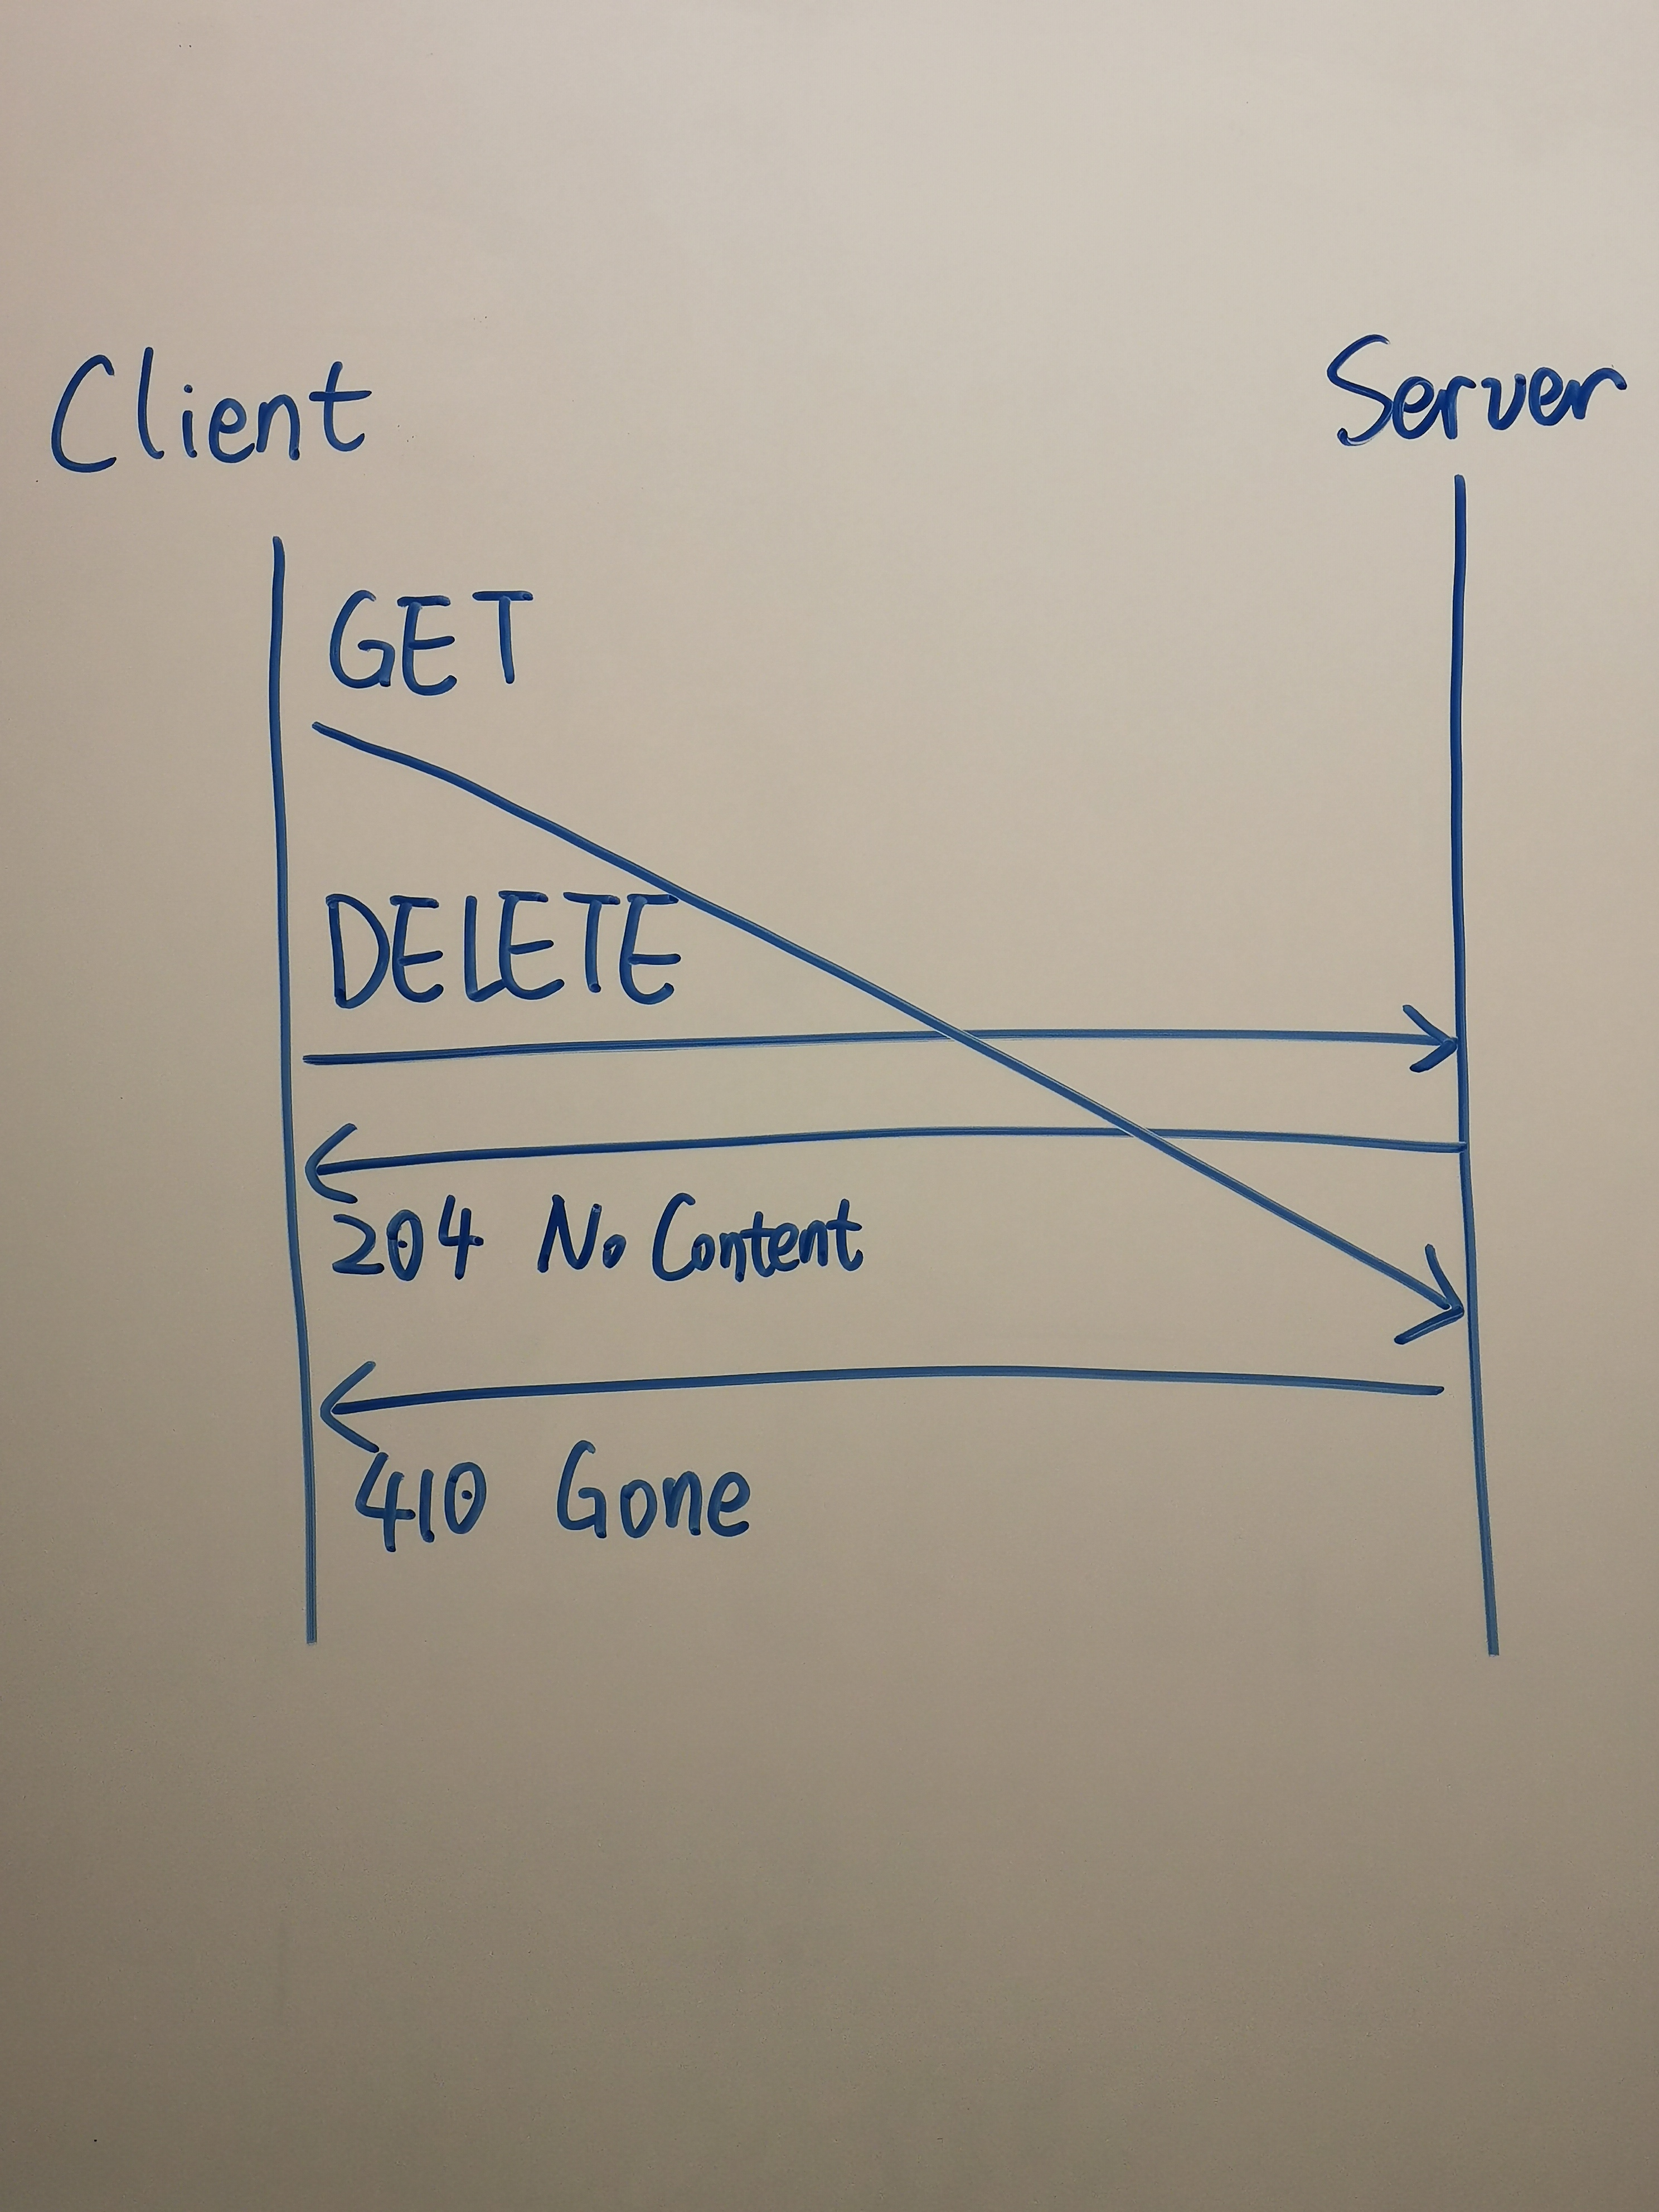
\includegraphics[width=\textwidth]{figures/trace}
  \end{minipage}
  \caption{Example client-side trace and its corresponding IR}
  \label{fig:trace}
\end{figure}

\section{Instantiating requests during runtime}
To instantiate a Jexp into request IR, the test harness substitutes all
occurences of ``$\Jref{\mathit{label}}{\mathsf{Jpath}}{\mathit{function}}$''
with its corresponding IR computed from the trace.  However, due to external
nondeterminism, the expected message label might be delayed and not available in
the trace.  Also, considering inter-execution nondeterminism, arrays in observed
messages might not have enough elements as expected in the Jexp.  In these
cases, the test harness searches for other labels in the trace and other
elements in the arrays as a fallback fulfillment to construct the request.

\lys{Todo: add instantiation algorithm.}

This idea of shrinking symbolic representations can be applied to scenarios
beyond networked servers.  For example, the HTTP testing experiment in
\autoref{sec:eval} has also used this technique to locate the bug pattern.
